\cotefile{157-4}
\scanpage{394}\mspage{118}
fondamentaux de $\mathrm{Cat}$) montre à
nouveau que si $W$ \inserted{loc. fond.} de $\mathrm{Cat}$ satisfait
à $\mathrm{Loc}(6'\mathrm{a},8,9)$, alors $\mathrm{HOT}_{W}$ est
un vrai dérivateur. On a vu de
plus dans 7.6 (page 111) que l'on
a \inserted{alors} $W=W^{\ast}_{\mathrm{HOT}_{W}}$, donc il s'ensuit
\deleted{que}
% slanted
\margin{Mais c'était sous l'hypothèse $\mathrm{Loc}(3\ \mathrm{bis})$ ! \unsure{Gare au|Erreur} cercle vicieux !}

\uline{Corollaire} 7.7.2 : \deleted{Les axiomes $\mathrm{Loc}(6\mathrm{a},8,9)$} \inserted{On a l'implication}
\[
\mathrm{Loc}(6'\mathrm{a},8,9)\Longrightarrow\mathrm{Loc}(1\ \mathrm{ter},\deleted{3\ \mathrm{bis}}).
\]
% slanted
\margin{pas prouvé, probablement faux}

Notons aussi, pour mémoire :

\uline{Corollaire} 7.7.3. Soit $(M,W)$ une
catégorie de modèles, associée à
une catégorie à cofibrations. Alors
sur le domaine $\mathrm{Dia}$ formé des
ens ordonnés finis, le prédérivateur
\inserted{$D={}$}$D_{M,W}$ satisfait aux axiomes
$\mathrm{Der}(1,2,3,4^{\unsure{\alpha|\prime|\wedge|\mathrm{a}}},5^{\alpha},\unsure{6|5|0}^{\alpha})$, et dualement. Donc
si $W$ est associée à la fois à une
structure de cofibrations et de fibrations,
$D$ est un dérivateur sur $\mathrm{Dia}$.
% archive sheet number: 393
\scanpage{395}\mspage{\unsure{119|149}}
alors la flèche de chgt. de base
\[
p^{\ast}f_{!}\longrightarrow f'_{!}\unsure{g|q}^{\ast}
\]
entre foncteurs $\mathrm{HOT}_{W}(X)\longrightarrow\mathrm{HOT}_{W}(S')$ est iso.

C'est pratiquement trivial, compte tenu, dans
le cas $f$ $W$-lisse, que si $Z$ sur $X$ est \unsure{$W$-lisse|lisse} sur $X$,
il l'est sur $S$ ; et dans le cas $p$ $W$-propre, en
utilisant le dernier énoncé (``oublié'') du (6),
p.~199.

7.8. Je termine en mettant en vedette
ce qui, à présent, me paraît la
\deleted{\unsure{résultat}} \inserted{substance} principale de tous ces ``rappels'', et
comme la quintessence de la théorie des localiseurs
fondamentaux développée jusqu'à présent :
\[
\left|\left\Vert\left\{\begin{aligned}
\mathrm{Loc}(3\ \mathrm{bis},)\deleted{\unsure{6\mathrm{a})}}&\Longrightarrow\mathrm{Der}(4^{\unsure{\alpha|\prime}},5^{\alpha})\\
\mathrm{Loc}(3\ \mathrm{bis},6\mathrm{a})&\Longrightarrow\mathrm{Der}(1,2,3,4^{\alpha},5^{\alpha},6^{\alpha})\\
\mathrm{Loc}(6'\mathrm{a},8,9)&\Longrightarrow\text{tous les axiomes des}\\
&\hphantom{\Longrightarrow{}}\text{dérivateurs}\quad(+\mathrm{Loc}(1\ \mathrm{ter})\deleted{3\ \mathrm{bis})})
\end{aligned}\right.\right.\right.
\]

Je considère les axiomes $\mathrm{Loc}(3\ \mathrm{bis})$,
$\mathrm{Loc}(8)$, $\mathrm{Loc}(9)$, comme des axiomes
``anodins'' --- tous les localiseurs \unsure{qu'on|qui}
\unsure{définit|définit.} par voie cohomologique ou homotopique
ordinaire, y satisfont. Il reste l'axiome
$\mathrm{Loc}(6\mathrm{a})$ \deleted{\unsure{des caté}} \inserted{ou $\mathrm{Loc}(6'\mathrm{a})$} \unsure{$W$-cofibrations|$W$-cofibration} (\unsure{formes|sens} faibles),
% archive sheet number: 394
\scanpage{396}\mspage{120}
qui visiblement joue un rôle crucial
\unsure{dans} la théorie de $\mathrm{HOT}_{W}$. Par contre,
les axiomes $\mathrm{Loc}(4)$\deleted{\unsure{,}} (\unsure{d'in-opposition|d'inopposition}),
$\mathrm{Loc}(5)$ (non-vacuité) et $\mathrm{Loc}(7)$\inserted{ et ses variantes}
(et bien sûr aussi $\mathrm{Loc}(6\mathrm{b})$) n'interviennent
absolument pas ! C'est particulièrement
impressionnant, en ce qui
concerne l'axiome \unsure{des|de} $W$-\unsure{fibrations|fibration}
$\mathrm{Loc}(7)$ et ses variantes (toutes équivalentes
à $\mathrm{Loc}(7)$ en présence de $\mathrm{Loc}(8)$, à la
seule exception de $\mathrm{Loc}(7\unsure{\mathrm{P}|\mathrm{F}})$). Comme
on a vu, $\mathrm{Loc}(7)$ n'est nullement impliqué
par $\mathrm{Loc}(6\mathrm{a},8,9)$, \deleted{tout au plus} ($\mathbb{W}_{\unsure{0|6}}$ n'y
satisfait pas), tout au plus se pourrait-il
que $\mathrm{Loc}(7\mathrm{F})$ le soit. Il en
est de $=$ de l'axiome de non-vacuité
$\mathrm{Loc}(5)$, comme on voit sur l'exemple
de $W=\mathrm{Fl}(\mathrm{Cat})$, qui satisfait à tous les
axiomes vus jusqu'à présent, à la seule exception
% archive sheet number: 395
\scanpage{397}\mspage{121}
de $\mathrm{Loc}(5)$. Quant à la question de l'indépendance
de l'axiome $\mathrm{Loc}(4)$ p.r.
à $\mathrm{Loc}(6\mathrm{a},8,9)$, nous allons examiner
ce genre de questions au \S{} suivant.

L'ensemble d'axiomes $\mathrm{Loc}(6'\mathrm{a},8,9)$ me
paraît à présent si important, que j'ai
\unsure{envie} de lui donner un nom, et
d'appeler \uline{localiseur} (fondamental) \uline{spécial}
sur $\mathrm{Cat}$,$^{\ast}$ un loc fond. qui y satisfait.
% slanted
\margin{J'hésite si je ne dois pas rajouter l'axiome $\mathrm{Loc}(3\ \mathrm{bis})$, qui assure que \unsure{l'on} \deleted{\illegible{1}} $W=W_{D}\deleted{\unsure{\mathrm{HOT}_{W}}}$, $D=\mathrm{HOT}_{W}$ ;}
Ce sont donc aussi ceux pour lesquels
nous savons que $\mathrm{HOT}_{W}$ est un
vrai \uline{dérivateur}. Si on ne peut
écarter comme ``pathologique'' une
structure aussi riche et délicate qu'un
dérivateur, il s'ensuit aussitôt que
l'on ne peut non plus écarter \deleted{\unsure{a}} les
localiseurs spéciaux dans $\mathrm{Cat}$ (même
si on affecte de regarder de haut les
% archive sheet number: 396
\scanpage{398}\mspage{122}
localiseurs fondamentaux généraux !). En
effet, $W$ se récupère de façon unique
à l'aide de $D=\mathrm{HOT}_{W}$, ou de \unsure{tout}
dérivateur équivalent à celui-ci,
comme l'ens des $D$-équivalences dans
$\mathrm{Cat}$:$^{\ast}$ c'est \unsure{la|le} localiseur fondamental
% slanted
\margin{Mais ceci n'est prouvé que moyennant $\mathrm{Loc}(3\ \mathrm{bis})$}
(correspondant à une notion d'équivalence
``universelle'', i.e. dans la catégorie $\mathrm{Cat}$
de tous les ``\unsure{engins|espaces}'' \deleted{\unsure{abs}}\unsure{élémentaires})
canoniquement associé à \unsure{ce|un} dérivateur.
Ce n'est donc nullement un localiseur
de référence \unsure{plus ou moins fin|fixé une fois}, tel $\mathbb{W}_{\infty}$,
qui est apte à jouer ce rôle !

Cela nous amène à nouveau à une
question du genre déjà soulevé : Si
$W$ \inserted{$\subset\mathbb{W}_{\infty}$} est le plus petit localiseur qui
satisfait à $\mathrm{Loc}(6'\mathrm{a},8)$ \inserted{(ou $\mathrm{Loc}(3\ \mathrm{bis},6'\mathrm{a},8)$)}, peut-on
dire a) que $W$ soit $=$ \uline{spécial} i.e.
% archive sheet number: 397
\scanpage{399}\mspage{123}
i.e. \unsure{satisfait|satisfasse} également $\mathrm{Loc}(9)$ (accessibilité ?),
et de plus $2^{\circ})$ a-t-on $W\ne\mathbb{W}_{\infty}$ ? Je
suis persuadé que c'est le cas (il
y a moins de mérite pour ce $W$-là
d'être $\ne W_{\infty}$, que pour le $\widetilde{\mathbb{W}}_{\infty}$
envisagé en \unsure{6.4} (p.~87)).

7.9. Oubli : la question 1 bis (p.~98),
sur l'existence d'une structure de Quillen
close sur $\mathrm{Cat}$, correspondant à $W$. Le
seul résultat que je connaisse dans
ce sens est celui de Thomason,
\deleted{\unsure{affirmant}} \inserted{construisant} explicitement une telle
structure de Quillen \inserted{(de plus propre)}, dans le cas $W=\mathbb{W}_{\infty}$.
Je n'ai pas vraiment regardé la démonstration
de Thomason, et ignore si celle-ci
peut s'étendre à des localiseurs fond. plus
généraux, par exemple à ceux satisfaisant
$\mathrm{Loc}(6'\mathrm{a},8,9)$. S'il en était ainsi, \unsure{cel|cela}
prouverait d'ailleurs que ces localiseurs
% archive sheet number: 398
\scanpage{400}\mspage{124}
ont assez de cofibrations et assez de fibrations,
donc qu'ils satisfont $\mathrm{Loc}(6\mathrm{a})$ et $\mathrm{Loc}(7\mathrm{F})$.
(Pour ce qui est de $\mathrm{Loc}(6\mathrm{a})$, il semble qu'on
puisse le prouver directement \inserted{très simplement}, cf \S{} suivant.)
Mais ici encore, il faudrait regarder quelques
exemples (équivalences homologiques ou cohomologiques,
$\mathbb{W}_{\unsure{n|m}}$ i.e. les $n$-équiv. d'homotopie.
et regarder déjà si $\mathrm{Loc}(7\mathrm{F})$ est satisfait.

Il ne \deleted{\unsure{sem}} semble pas que le th. de
Thomason ait été \inserted{jusqu'à présent} ou doive être très utile,
\deleted{\unsure{plutôt|théori}} techniquement parlant. Psychologiquement,
je crois qu'il a été important,
pour donner confiance que $\mathrm{Cat}$ est vraiment
une excellente catégorie de modèles
pour $\mathrm{Hot}$. J'ai été vraiment enchanté et
stimulé d'apprendre ce théorème. Mais
la notion d'application de Dwyer (que j'ai
apprise \inserted{en 1983} dans l'article de Thomason) a
été, techniquement, beaucoup plus \unsure{importante|important}
pour moi : c'était exactement ce qui
manquait à ma panoplie de notions et d'\unsure{intuitions}
``homotopiques'' dans $\mathrm{Cat}$ ....
% archive sheet number: 399
\scanpage{402}\mspage{\textcircled{1}}
% archive sheet number: 401
XV p.~119
\diagram{\begin{tikzcd}[ampersand replacement=\&,column sep=small]
X \arrow[rr] \arrow[dr] \& \& Y \arrow[dl]\\
\& S \&
\end{tikzcd}}
\[
\begin{aligned}
\mathrm{I}^{\circ}/)\quad\text{\textcircled{A}}\quad\mathrm{Loc}(8)&\Longrightarrow\mathrm{Loc}(1\ \mathrm{bis})\\
\text{\textcircled{B}}\quad\mathrm{Loc}(6'\mathrm{a},8,9)&\Longrightarrow
\mathrm{Loc}(1\ \mathrm{ter},\underset{\substack{\vert\\\inserted{\text{\unsure{non|voir} }4\mathrm{b}}}}{4\mathrm{a}},6\mathrm{a})
\end{aligned}
\]
\margin{$\swarrow$ il suffit $=$ $\mathrm{Loc}(6'\mathrm{a},8\deleted{\unsure{)}}\mathrm{bis})$}

Cela implique-t-il \deleted{$\mathrm{Loc}(3\ \mathrm{bis})$} ?
\[
W=W_D,\ \text{\unsure{ou|où} }D=\mathrm{HOT}_{W}\ ?
\]
J'en doute ! (\unsure{Histoire} de triples de Quillen très spéciaux ?)
Et je doute aussi, par suite, que ça implique $\mathrm{Loc}(3\ \mathrm{bis})$.

\figure{\begin{tikzpicture}\draw (0,0) -- (0.75,-1.1);\draw (0.94,-1.34) -- (0.99,-1.43);\end{tikzpicture}}
\[
\deleted{\unsure{\mathrm{II}}}\mathrm{I}\quad
\left\{\begin{aligned}
\mathrm{Loc}(6'\mathrm{a})&\Longrightarrow\mathrm{Loc}(4\mathrm{a}_{\unsure{0|\mathrm{o}}})\\
\mathrm{Loc}(6'\deleted{\unsure{\mathrm{a}}}\mathrm{b})&\Longrightarrow\mathrm{Loc}(4\deleted{\unsure{\mathrm{a}_{0}}}\mathrm{b})\\
\mathrm{Loc}(6\deleted{\unsure{\prime}},8)&\Longrightarrow\mathrm{Loc}(4)
\end{aligned}\right.
\]
\[
\left\{\begin{aligned}
\mathrm{Loc}(7D_{W_{\unsure{\omega|\infty|0}}})&\Longrightarrow\mathrm{Loc}(4\mathrm{b})\\
\deleted{\unsure{\mathrm{Loc}(3}}\ &\\[-2pt]
\deleted{\mathrm{Loc}(7D_{W_{\omega}},} &\\
\mathrm{Loc}(6'\mathrm{a},7,8)&\Longrightarrow\mathrm{Loc}(4)\\
\deleted{\mathrm{Loc}(3\ \mathrm{bis})}&
\end{aligned}\right.
\]
\[
\unsure{\mathrm{II}_{\mathrm{e}}|\mathrm{III}_{\mathrm{e}}}\quad
\left\{\begin{aligned}
\mathrm{Loc}(3\ \mathrm{bis})&\Longrightarrow\deleted{\unsure{\mathrm{D}}}\mathrm{Loc}(4\mathrm{a}_{0})\\
\mathrm{Loc}(3\ \mathrm{bis},8)&\Longrightarrow\deleted{\unsure{\mathrm{D}}}\mathrm{Loc}(4\mathrm{a})\\
\mathrm{Loc}(3\ \mathrm{bis},7,8)&\Longrightarrow\deleted{\unsure{\mathrm{D}}}\mathrm{Loc}(4)
\end{aligned}\right.
\]
\[
\mathrm A\left|\begin{aligned}
\mathrm{Loc}(4\mathrm{a}_{0}):&\ \text{impliqué par }\mathrm{Loc}(6'\mathrm{a}),\ \mathrm{Loc}(3\ \mathrm{bis})\\
\mathrm{Loc}(4\mathrm{a}):&\ \text{impliqué par }\mathrm{Loc}(6'\mathrm{a},8\deleted{\mathrm{bis}})\deleted{\unsure{9}},\ \mathrm{Loc}(3\ \mathrm{bis},8\deleted{\mathrm{bis}})\\
\mathrm{Loc}(4\mathrm{b}):&\ \text{impliqué par }\mathrm{Loc}(6'\mathrm{b})\ (\text{donc par }\mathrm{Loc}(6)),\ \mathrm{Loc}(7D_{W_{\omega}})\\
\mathrm{Loc}(4):&\ \text{impliqué par }\mathrm{Loc}(6\deleted{\unsure{\prime}},8\deleted{\mathrm{bis}}),\
\mathrm{Loc}(6'\mathrm{a},7\deleted{\unsure{D_{W_{\omega}}}},8\deleted{\mathrm{bis}}),\\
&\quad\deleted{[\mathrm{Loc}(3\ \mathrm{bis},6'\mathrm{b},8\mathrm{bis})]}\deleted{\unsure{,}}
\mathrm{Loc}(3\ \mathrm{bis},7\deleted{\unsure{D_{W_{\omega}}}},8\deleted{\mathrm{bis}})
\end{aligned}\right.
\]
\scanpage{403}
% Two long oblique cancellation strokes span the diagrams and text above the last diagram.
\deleted{\diagram{\begin{tikzcd}[ampersand replacement=\&]
X_0 \arrow[r,thick] \arrow[d,no head] \& X_1 \arrow[d,thick] \&\\
X_2 \arrow[r,thick] \& \unsure{\mathscr{X}|\mathcal{X}} \arrow[r] \& X_3
\end{tikzcd}}
\diagram{\begin{tikzcd}[ampersand replacement=\&]
X_0 \arrow[r,no head] \arrow[d] \& X_1 \arrow[d,no head]\\
X_2 \arrow[r,no head] \& {}
\end{tikzcd}}

a) $\mathscr{X}_{D}$ est \deleted{une $W$-somme} isomorphe \inserted{dans $\mathrm{Hot}_{W}$} à la
\deleted{carré $W$-} somme \deleted{\unsure{co}}amalgamée \deleted{\unsure{du}}
$W$-homotopique du \deleted{$X_0,X_1,X_2$} diagramme
\diagram{\begin{tikzcd}[ampersand replacement=\&,row sep=tiny]
\& X_1\\
X_0 \arrow[ur] \arrow[dr] \&\\
\& X_2
\end{tikzcd}}
(Moyennant $\mathrm{Loc}(6\mathrm{a})$

b) Si on a un carré commutatif
\diagram{\begin{tikzcd}[ampersand replacement=\&]
X_0 \arrow[r,no head] \arrow[d,no head] \& X_1 \arrow[d]\\
X_2 \arrow[r] \& Y
\end{tikzcd}}
, d'où $\inserted{\varphi_{\unsure{Q|\alpha}}:}\mathscr{X}_{\deleted{\unsure{Q}}D}\longrightarrow Y$,
alors $\mathrm{hot}_{W}(\varphi_{Q})$ s'identifie \inserted{(via \unsure{a)|a})} à la flèche
canonique \deleted{$\unsure{f}_{W}$} allant de la somme
amalgamée $W$-homotopique de $D$ vers $Y$
(ds $\mathrm{Hot}_{W}$).}

\diagram{\begin{tikzcd}[ampersand replacement=\&]
X_0 \arrow[r] \arrow[d] \& X'_1 \arrow[d] \&\\
X'_2 \arrow[r] \& \mathscr{X} \arrow[r,very thick,"\varphi_{Q}"] \& Y
\end{tikzcd}}
% archive sheet number: 402
\scanpage{404}\mspage{\textcircled{2}}
\handwritten{$\mathrm{Cat}\longrightarrow\Delta^{1}$ \unsure{définit} \deleted{\unsure{dérivateur}} \inserted{localiseur} $\mathbb W_{\unsure{?|\varnothing}}$
\[
\mathrm{Loc}(1\ \mathrm{ter},2,3\ \mathrm{bis},4\mathrm{a},
\deleted{\unsure{,}5},\underset{\text{\inserted{\uline{non b}}}}{6^{\unsure{\ast|\prime}}\mathrm{a}},
\deleted{\unsure{7\mathrm{F}_{\mathrm{f}}}},8,9)
\]
% slanted
\margin{manque $\mathrm{Loc}(4\mathrm{b},5,6'\mathrm{b})\deleted{\unsure{,7}}\ \downarrow\unsure{Y}$\\
$\mathrm{Loc}(4\mathrm{b},5,6'\mathrm{b},7\deleted{\unsure{\mathrm F}})$}

\diagram{\begin{tikzcd}[ampersand replacement=\&,column sep=small]
X \arrow[rr,thick] \arrow[dr,no head] \& \& Y \arrow[dl,no head]\\
\& S \&
\end{tikzcd}}
\[
\begin{aligned}
X_{/s}\longrightarrow Y_{/s}&\quad\in W\\
\Longrightarrow\quad X\mathbin{-}Y&\quad\in W .
\end{aligned}
\]
i.e. si $X=\varnothing$, $Y\ne\varnothing$, $\exists\,s\in S$ tel
que $X_{/s}\mathbin{-}Y_{/s}$ \unsure{non} ds $W$.

Si $Y\ne\varnothing$, $\exists\,s\in S$ tel que $Y_{/s}\ne\varnothing$,
mais $X_{/s}=\varnothing$, donc $X_{/s}\mathbin{-}Y_{/\unsure{s|0|b}}$ non ds $W$,
\diagram{\begin{tikzcd}[ampersand replacement=\&]
\deleted{\unsure{X\simeq Y}_{W}} \arrow[d,no head] \& X'\ne{} \arrow[d]\\
\varnothing \arrow[r,very thick,"\mathrm{Fib}_{W}"'] \& X\\
\& \deleted{\unsure{Z\simeq}}
\end{tikzcd}}
\diagram{\begin{tikzcd}[ampersand replacement=\&]
\& X_0 \arrow[d,very thick,"\in W?"'] \& \& X \arrow[d,"\in W"]\\
\deleted{X_0\amalg X} \& S_0 \& \amalg\ S_1= \& S
\end{tikzcd}}
Si $S_1\ne\varnothing$, alors $X=S_1\mathbin{-}S$ est $\in W$,
mais $X_0=\varnothing\mathbin{-}S_0$ n'est pas ds $W$,
si $X_0\ne\varnothing$.
\diagram{\begin{tikzcd}[ampersand replacement=\&]
X_{i}\arrow[r] \& Y_{i}\\
X\arrow[r,thick] \& Y
\end{tikzcd}}
\diagram{\begin{tikzcd}[ampersand replacement=\&]
\deleted{X_0}\varnothing \arrow[r,"W"] \arrow[d] \& X_1\ne\varnothing \arrow[d,no head]\\
\deleted{X_2}\varnothing \arrow[r,"{\deleted{\unsure{W}}}"] \& X\ne\varnothing
\end{tikzcd}}
\diagram{\begin{tikzcd}[ampersand replacement=\&,row sep=small,column sep=small]
\& \varnothing \arrow[rr,no head] \arrow[dl,no head] \arrow[dd,no head,dashed,"W" description] \& \& \varnothing \arrow[dl,no head] \arrow[dd,no head]\\
\varnothing \arrow[rr,no head] \arrow[dd,no head,"W"'] \& \& \varnothing \arrow[dd,no head,"W"] \&\\
\& \varnothing \arrow[rr,no head,dashed] \arrow[dl,no head] \& \& X\ne\varnothing \arrow[dl,no head]\\
\varnothing \arrow[rr,no head] \& \& \varnothing \&
\end{tikzcd}}}
% letterhead
% The printed stationery is upside down in relation to the handwritten diagrams.
MINISTERE DE L'EDUCATION NATIONALE \hfill AVIGNON, le\\
ACADEMIE D'AIX-MARSEILLE\\
\rule{1.3cm}{0.3pt}\\
Inspection Académique \hfill L'Inspecteur d'académie,\\
de Vaucluse \hfill directeur des services départementaux\\
\rule{1.3cm}{0.3pt}\hfill de l'Education Nationale de Vaucluse,\\
Tél. : 90 82 99 76\\
Référence : Secrétariat n\textsuperscript{o} \hfill à M
\handwritten{\diagram{\begin{tikzcd}[ampersand replacement=\&]
\varnothing \arrow[r,thick] \arrow[d,no head] \& X_1 \arrow[d]\\
X_2 \arrow[r] \& X_1\amalg X_2
\end{tikzcd}}}
% archive sheet number: 403
\scanpage{405}
% The handwriting is inverted relative to the archive number.
% One continuous oblique cancellation crosses the diagrams marked below.
\deleted{\diagram{\begin{tikzcd}[ampersand replacement=\&,column sep=small]
U \arrow[d,"W"'] \& \overset{W}{\subset} \& \bar U \arrow[d,"W"] \& \subset \& X \arrow[d,no head] \& \supset \& Y \arrow[d,Rightarrow]\\
U' \& \underset{W}{\subset} \& \bar U' \& \subset \& X' \& \supset \& Y
\end{tikzcd}}}
\[
\bar U\cap Y=\dot Y
\]
\margin{\uline{p.~124,125} / p.~\unsure{264|254}\\ à faire \unsure{rajout}\\ \deleted{$\unsure{X}_{0}$}}

\deleted{\diagram{\begin{tikzcd}[ampersand replacement=\&,row sep=small,column sep=small]
\&Y\arrow[rrdd]\arrow[dd,no head]\&\&\\
\dot Y\arrow[ur]\arrow[dr,thick]\arrow[dddd,no head]\&\&\&\\
\&\bar U\arrow[rr]\arrow[dddd]\&\&X\arrow[dddd,no head,"W"]\\
\&\&\&\\
\&Y'\arrow[rrdd]\&\&\\
\dot Y\arrow[ur]\arrow[dr,thick]\&\&\&\\
\&\bar U'\arrow[rr]\&\&X'
\end{tikzcd}}}
\[
X_1
\]
\deleted{\diagram{\begin{tikzcd}[ampersand replacement=\&,row sep=tiny,column sep=small]
\&\&X_1\&\&\\
\displaystyle\int\&X_0\arrow[ur]\arrow[dr]\&{}\arrow[rr,very thick]\&\&X\\
\&\&X_2\&\&
\end{tikzcd}}}
\diagram{\begin{tikzcd}[ampersand replacement=\&,row sep=small,column sep=small]
\&X\arrow[dr,no head]\&\\
S\arrow[ur,no head,"\mathrm{Cof}_{W}"]\arrow[dr,no head,"\mathrm{cof}_{W}"']\arrow[dd]\&\&\bullet\\
\&Y\arrow[ur,no head]\&\\
S'\&\&\mathrm{Fib}_{W}\cap W
\end{tikzcd}}
\deleted{\diagram{\begin{tikzcd}[ampersand replacement=\&]
X_{0y}\arrow[r,no head]\arrow[d]\&X_{1y}\\
e\&
\end{tikzcd}}}
\deleted{\diagram{\begin{tikzcd}[ampersand replacement=\&,column sep=small]
Z\arrow[rr,very thick]\arrow[dr,thick]\&\&Z\arrow[dr,dashed]\&\\
\&e\arrow[rr,dash dot]\&\&\unsure{\circ|0}
\end{tikzcd}}}

\figure{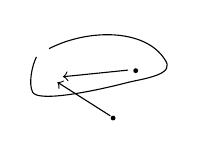
\begin{tikzpicture}[scale=.7]
\draw (-1.08,.43) .. controls (-.38,.79) and (.66,.8) .. (1.02,.23) .. controls (1.21,-.03) and (.72,-.1) .. (.36,-.18) .. controls (-.25,-.34) and (-1.28,-.55) .. (-1.38,-.36) .. controls (-1.46,-.21) and (-1.39,.13) .. (-1.31,.28);
\fill (.49,.03) circle (1.25pt); \fill (.08,-.83) circle (1.25pt);
\draw[->] (.35,.04)--(-.83,-.08); \draw[->] (.03,-.79)--(-.93,-.18);
\end{tikzpicture}}

\deleted{\diagram{\begin{tikzcd}[ampersand replacement=\&,row sep=small,column sep=small]
\&X_{\unsure{1}}\arrow[dr]\arrow[ddd,no head,"W"']\&\\
X_0\arrow[ur,"\alpha_1"]\arrow[dr,"\alpha_2"']\arrow[ddd,"\mathrm{id}"']\&\&\unsure{\mathscr X|\mathcal X}\arrow[ddd,"\mathrm{id}"]\\
\&X_2\arrow[ur]\arrow[ddd,"W"]\&\\
\&\overset{\unsure{+|\downarrow}}{X'_1}\arrow[dr,dash pattern=on 2pt off 1pt on 2pt off 1pt on 2pt off 1pt on 120pt off 0pt]\&\\
X_0\arrow[ur,no head,"\alpha'_1"]\arrow[dr,"\alpha'_2"']\&\&\mathscr X\\
\&X'_2\arrow[ur]\&
\end{tikzcd}}}
% archive sheet number: 404
\scanpage{406}
% letterhead
MINISTERE DE L'EDUCATION NATIONALE \hfill AVIGNON, le\\
ACADEMIE D'AIX-MARSEILLE\\
\rule{1.3cm}{0.3pt}\\
Inspection Académique \hfill L'Inspecteur d'académie,\\
de Vaucluse \hfill directeur des services départementaux\\
\rule{1.3cm}{0.3pt}\hfill de l'Education Nationale de Vaucluse,\\
Tél. : 90 82 99 76\\
Référence : Secrétariat n\textsuperscript{o} \hfill à M

\handwritten{\diagram{\begin{tikzcd}[ampersand replacement=\&,column sep=small]
\&\&\unsure{\xi|\zeta}\\
\deleted{\unsure{b}}\arrow[r,shift left=3pt,"{\deleted{\diagup\!\diagup\!\diagup}}" description]\arrow[r,shift right=2pt]\&c\arrow[ur,thick]\&
\end{tikzcd}}
\diagram{\(\underbrace{\begin{tikzcd}[ampersand replacement=\&,column sep=small,row sep=small]
\&{}\arrow[r,draw=none,no head,"{\overbrace{\hphantom{\quad A\quad B\quad}}^{\Psi}}" description]\&{}\\
\&\& B\\
\xi \arrow[r,shift left] \arrow[r,shift right] \& A \arrow[ur] \arrow[dr]\&\\
\&\& C
\end{tikzcd}}_{Z}\)}
\diagram{\(\dfrac{\xi\backslash\Psi=\begin{tikzcd}[ampersand replacement=\&,row sep=small]
A_1\arrow[r]\arrow[dr,dash pattern=on 6pt off 3pt on 70pt off 0pt]\& B'\\
A_2\arrow[ur]\arrow[r]\& C'
\end{tikzcd}}{\deleted{\unsure{\Psi'}}\unsure{\vert}S\ (\approx S^{1})}\)}
\diagram{\begin{tikzcd}[ampersand replacement=\&,execute at end picture={\draw ([xshift=-.38cm,yshift=.68cm]immx.north) .. controls +(.45,.04) and +(-.6,.08) .. ([xshift=.95cm,yshift=.26cm]immx.north) .. controls +(.45,-.06) and +(-.35,.1) .. ([xshift=1.83cm,yshift=.29cm]immx.north) .. controls +(.32,-.02) and +(0,.2) .. ([xshift=2.02cm,yshift=-.13cm]immx.north);\draw ([xshift=1.98cm,yshift=.57cm]immxb.east) .. controls +(.1,-.46) and +(.45,.47) .. ([xshift=1.18cm,yshift=-.27cm]immxb.east); }]
\Psi\arrow[r]\arrow[d,"\text{\unsure{imm.} fermée}"']\& |[alias=immx]|X\arrow[d,thick,"\text{imm. fermée}"]\\
Z\arrow[r,no head]\&|[alias=immxb]|X'\ \text{ou } Z'
\end{tikzcd}}
\diagram{\begin{tikzcd}[ampersand replacement=\&,row sep=small]
a\arrow[r,shift left]\arrow[r,no head,shift right]\&b
\end{tikzcd}}
\diagram{\begin{tikzcd}[ampersand replacement=\&,row sep=tiny]
\&b\arrow[dr]\&\\
\unsure{-|a}\arrow[ur]\arrow[dr,very thick]\&\&d\\
\&\unsure{b|c}\arrow[ur]\&
\end{tikzcd}\quad
$\displaystyle\left|\underset{x\in X}{\underrightarrow{\lim}}\ {}^{\unsure{\prime}}\mathrm{Hom}(\xi,x)\right.$}

\deleted{Si \unsure{les} \unsure{$\xi\backslash X$} \unsure{sont|est} \uline{\unsure{fblt} \unsure{filtrantes|filtrante}}, $X$ \unsure{a-mê\-me}
alors $X$ est filtrante ?}

\diagram{\begin{tikzcd}[ampersand replacement=\&,column sep=small]
\Psi\arrow[r,hook,"\text{ferm}"]\arrow[d,thick,"{\deleted{\unsure{f}}}"']\&Z\arrow[r,"o"]\arrow[d,thick,"g"]\&\xi\\
X\arrow[r,"\text{ferm}","g"']\&\underset{\text{ou }X'}{Z'}\arrow[r,"o"]\&\xi'
\end{tikzcd}}
\deleted{\diagram{\begin{tikzcd}[ampersand replacement=\&,column sep=small]
(\unsure{\xi\rightrightarrows A})\arrow[r]\arrow[d,"\text{\unsure{imm. ferm.}}"']\&\Psi\arrow[r]\arrow[d,thick]\&X\\
(\xi\rightrightarrows A)\arrow[r]\&Z\&
\end{tikzcd}}}
\diagram{\begin{tikzcd}[ampersand replacement=\&,column sep=small]
\underline{\underline{\xi}}\arrow[r]\&x_0\arrow[d,no head]\&\\
\&\varphi(x_0)\arrow[r]\&\underline{\underline{x}}
\end{tikzcd}}
\[
\mathrm{Hom}(\xi',x)\overset{(?)}{=}\unsure{\Pi|\pi}_0(\deleted{\unsure{z}}\xi\backslash\Psi/\deleted{\unsure{\xi}}x)^{\unsure{\prime\prime}}
\]
\margin{$\underline{\Pi_0(S/x)}\hbox{\tikz[baseline=0pt]{\draw (0,-.08) .. controls (.18,-.09) and (.23,-.15) .. (.24,-.43);}}$}

\uline{NB}\quad
$\boxed{g_{\unsure{!|1}}(e_{Z^{\unsure{\wedge|\prime}}})=e_{Z'}}$
\quad i.e. $\underset{X}{\underrightarrow{\lim}}\ \Pi_0(\unsure{S| \xi}/x)\unsure{\simeq|\ne|\approx} e$}
% archive sheet number: 405
\scanpage{407}
\[
X\ \text{tot. }\mathbb W_{\unsure{1|9}}\text{-asph.}\ \Longleftrightarrow\ X\ \text{filtrante}\ ?!
\]
\uline{Cor}\quad \deleted{\unsure{X}} Soit $W\subset\mathbb W_{1}$ \deleted{\unsure{identité}} Si $X$ tot $W$-asph,
$X$ filtrante, et inversement si $\mathrm{Loc}(8)$

\deleted{$a\unsure{,|\to}b$ dans $X$, $\exists\,c$ tel $a\longrightarrow c,b\unsure{\longrightarrow|-}c$
\unsure{Supposons} l'inverse, et \unsure{considérons|conditions}}

a) $X$ est $0$-connexe \quad OK

b) Pour
\diagram{\begin{tikzcd}[ampersand replacement=\&,row sep=tiny]
\&b\\
\unsure{a|\bullet}\arrow[ur,no head]\arrow[dr,no head]\&\\
\&c
\end{tikzcd}}
dans $X$, on peut
compléter en
\diagram{\begin{tikzcd}[ampersand replacement=\&,row sep=tiny]
\&b\arrow[dr]\&\\
a\arrow[ur]\arrow[dr,no head]\&\&d\\
\&c\arrow[ur]\&
\end{tikzcd}}
comm. ?

\diagram{\begin{tikzcd}[ampersand replacement=\&,row sep=tiny]
b\arrow[dr,very thick]\&\\
\&\deleted{\unsure{\varepsilon}}\unsure{\xi|\zeta}\\
c\arrow[ur,very thick]\&
\end{tikzcd}}
\diagram{\begin{tikzcd}[ampersand replacement=\&]
\unsure{\varepsilon|E}\arrow[r]\arrow[d,"\text{\uline{imm ouv.}}"']\& X\arrow[d,"j"',"\text{imm ouverte}"]\\
\Phi\arrow[r]\&X'
\end{tikzcd}}
\[
\left\{\begin{aligned}
\mathrm{Hom}(\xi,x)&=\varnothing\\
\mathrm{Hom}(x,\xi)&=\mathrm{Hom}(x,b)\\
&\qquad\amalg\,\mathrm{Hom}(x,c)
\end{aligned}\right.
\]
\diagram{\begin{tikzcd}[ampersand replacement=\&,row sep=tiny]
\&b\arrow[dr]\&\\
x\arrow[ur,no head]\arrow[dr,no head]\&\&\xi\\
\&c\arrow[ur,no head]\&
\end{tikzcd}}
\[
\mathrm{Hom}(\xi,\xi)=e
\]
\diagram{\begin{tikzcd}[ampersand replacement=\&]
y\arrow[r]\&x\arrow[r]\&\xi
\end{tikzcd}}
\[
\begin{aligned}
\underset{X^{\wedge}}{\underrightarrow{\lim}}\ \deleted{\unsure{a}}\unsure{j(x)|y(x)|g(x)}&=e_{\unsure{X'|X1|X_1}}\\
\unsure{y_{\mathrm{ens}}(\xi)|j_{\mathrm{ens}}(\xi)|j\mathrm{ens}(\xi)}&=\deleted{\mathrm{Hom}(x,b)\amalg\mathrm{Hom}(x,c)}\inserted{\varnothing}\\
\underrightarrow{\lim}\ \varnothing&=\varnothing
\end{aligned}
\]
% archive sheet number: 406
\scanpage{408}
\[
\unsure{H1|H^{1}|H_{1}}(\unsure{Z|z}^{\unsure{\prime|1}},\mathbb{Q})\ne\varnothing\quad\text{si}\quad
\nexists d\quad\deleted{\unsure{\text{com}}}\quad\unsure{\text{comm}}
\]
\diagram{\begin{tikzcd}[ampersand replacement=\&]
 \& b\arrow[dr,no head] \& \\
 a\arrow[ur,no head]\arrow[dr] \& \& d\\
 \& c\arrow[ur,no head] \&
\end{tikzcd}}

\diagram{\begin{tikzcd}[ampersand replacement=\&]
\cdot\arrow[r,bend left=42]\arrow[r,bend right=42] \& \cdot
\end{tikzcd}}

\diagram{\begin{tikzcd}[ampersand replacement=\&]
\unsure{\xi|\zeta}\arrow[r,bend left=12]\arrow[r] \& y\\
{}\arrow[dr,"{\deleted{\diagup\!\diagup\!\diagup}}" description] \&\\
\deleted{\cdot} \& e\arrow[uu]\\
{}\arrow[ur,"{\deleted{\diagup\!\diagup}}" description] \&
\end{tikzcd}}

\diagram{\begin{tikzcd}[ampersand replacement=\&]
 A_1\arrow[r,"u"] \& B'\arrow[dd,no head]\\
 A_2\arrow[ur] \& \\
 \underset{a}{\bullet}\arrow[r,"\alpha"] \& b
\end{tikzcd}}

\[
S_{/a}\unsure{\longrightarrow|\text{---}}S_{/b}
\qquad
\begin{aligned}
\alpha_{\unsure{1|2}}&\in S_{/b} & A_1,&\quad\alpha\\
\alpha_2&\in S_{/b} & A_2,&\quad\unsure{a|\alpha}\\
\alpha_0&\in S_{/b} & B',&\quad\mathrm{id}_b
\end{aligned}
\]

\[
\begin{aligned}
\mathbb{W}_n^{H}&\quad\mathbb{W}_n^{\deleted{\unsure{P|R}}\unsure{K|k}}\\
\mathbb{W}_1^{k}&
\end{aligned}
\qquad u
\]

\diagram{\begin{tikzcd}[ampersand replacement=\&,column sep=small]
\unsure{p|\varphi}(\unsure{\cdot}A_1)=a\arrow[rr,no head,"p(u)=\alpha"]\arrow[d]\arrow[ddr,no head,"\alpha"] \& \& p(B')=b\arrow[d]\arrow[ddl,no head,"\mathrm{id}"']\\
{} \& \& {}\\
 \& b \&
\end{tikzcd}}
% archive sheet number: 407
\scanpage{409}
% letterhead
\noindent\begin{tabular}{@{}l@{\qquad}l@{}}
MINISTERE DE L'EDUCATION NATIONALE & AVIGNON, le\\
ACADEMIE D'AIX-MARSEILLE &\\
\multicolumn{1}{c}{\rule{1.1cm}{0.4pt}} &\\
Inspection Académique & L'Inspecteur d'académie,\\
de Vaucluse & directeur des services départementaux\\
\multicolumn{1}{c}{\rule{1.1cm}{0.4pt}} & de l'Education Nationale de Vaucluse,\\
Tél. : 90 82 99 76 &\\
Référence : Secrétariat n\textsuperscript{o} & à M
\end{tabular}

% Long diagonal from the telephone line through the formulae to the foot.
\handwritten{\deleted{%
\diagram{\begin{tikzcd}[ampersand replacement=\&]
S\arrow[r,"\Psi"] \& X
\end{tikzcd}}
\[
\unsure{\Pi|\pi}_0(S_{/x})\qquad\deleted{\unsure{(\Psi)|\xi}}
\]
\[
\underrightarrow{\lim}\ \Pi_0(S_{/\unsure{x|n}})
\]
\[
\begin{aligned}
x_1&=b,\quad s_1=B',\quad u_1=\mathrm{id}_b\\
x_2&=c,\quad s_2=C',\quad u_2=\mathrm{id}_c
\end{aligned}
\]
\[
j_!(e_{X^{\wedge}})(\unsure{\xi|\zeta}')\ni\xi_1,\xi_2\hbox{\tikz[baseline=0pt]{\draw (0,0) .. controls (.43,.05) and (.57,.79) .. (.39,1.07);}}
\]
\deleted{\unsure{$b$}}\quad\deleted{\unsure{h}}\unsure{homologie} de \unsure{dim} $\leq 1$
}

\figure{\begin{tikzpicture}\draw[gray,->,thin] (0,0)--(0,.42);\end{tikzpicture}}
\diagram{\begin{tikzcd}[ampersand replacement=\&]
 \& \& B'\\
 A_2\arrow[urr]\arrow[dr,no head] \& A_1\arrow[ur]\arrow[d,no head] \&\\
 \& a\arrow[r,"\deleted{\unsure{a|\alpha}}" description] \& b\arrow[uu]
\end{tikzcd}}
\[
S_{/b}\qquad \unsure{A_1|A.}
\]

\deleted{\unsure{$A$}}\qquad\deleted{\unsure{$b_1 b_2$}}

\diagram{\begin{tikzcd}[ampersand replacement=\&]
 \& b\\
 a\arrow[ur]\arrow[dr] \&\\
 \& c
\end{tikzcd}}

\deleted{\unsure{$A_1 A_2$}}$)$

\deleted{%
\[
\Pi_0(S_{/\unsure{a|\bullet}})
\]
\diagram{\begin{tikzcd}[ampersand replacement=\&,cells={nodes={inner sep=2pt}}]
 \& \& |[draw,ellipse]| B' \&\\
 \& \& b\arrow[r] \& x\\
 |[draw,ellipse]| A_1\text{ ou }A_2 \& a\arrow[ur]\arrow[dr]\arrow[rr,shift left=2pt,"A_1"]\arrow[rr,shift right=2pt,"A_2"'] \& \& z\\
 \& \& c\arrow[r] \& y\\
 \& \& |[draw,ellipse]| C' \&
\end{tikzcd}}
}

\deleted{\unsure{$a\,x$}}\qquad\deleted{\unsure{$a\longrightarrow$}}}
% archive sheet number: 408
